\section{Modeling Techniques} \label{ch:modeling_techniques}

In the previous chapters, we have explored various modeling techniques that are essential for solving complex optimization problems.
We began by discussing the decoupling of variables using quantifier elimination, a powerful method that simplifies the problem by reducing the number
of variables involved.
This technique is particularly useful in scenarios where the relationships between variables are intricate and non-linear.

Next, we examined convex relaxations, specifically focusing on McCormick envelopes for bilinear terms.
Convex relaxations are important for transforming non-convex problems into convex ones, which are easier to solve.
McCormick envelopes provide a way to approximate bilinear terms with convex functions, thereby enabling the use of efficient convex optimization
algorithms.

In this section, we present a collection of commonly used modeling methods for convex programming.
These methods serve as a practical guide for formulating and solving convex optimization problems.

\subsection{Soft Constraints}

Soft constraints are used in optimization problems where certain constraints can be violated to some extent, but with a penalty.
This is in contrast to hard constraints, which must be strictly satisfied.
Soft constraints are particularly useful in real-world scenarios where it is often impractical to meet all constraints perfectly.

To incorporate soft constraints into a convex optimization problem, we introduce slack variables and a penalty term in the objective function.
The slack variables measure the extent of constraint violation, and the penalty term ensures that violations are minimized.

Consider a constraint of the form \( g(x) \leq 0 \).
To make this constraint soft, we introduce a slack variable \( s \geq 0 \) and modify the constraint to \( g(x) \leq s \).
We then add a penalty term \( \lambda s \) to the objective function, where \( \lambda \) is a positive weight that controls the trade-off between
minimizing the original objective and satisfying the constraint.

The modified optimization problem can be written as:
\begin{align*}
	\min_{x, s} \quad       & f(x) + \lambda s \\
	\text{subject to} \quad & g(x) \leq s      \\
	                        & s \geq 0
\end{align*}

By adjusting the value of \( \lambda \), we can control the degree to which the soft constraint is enforced.
A larger \( \lambda \) places more emphasis on satisfying the constraint, while a smaller \( \lambda \) allows for greater flexibility in violating
the constraint.

\subsection{Auxiliary Variables}

Auxiliary variables can be used for modeling in many ways.
In our models we are the defining the road with as a function over $s$ the distance along the road.
One common part objective may be to minimize the offset to the center of the road.
The first formulation that may come to mind is: \[ \min g(x, u) + \left( n - \frac{\overline{n}(s) - \underline{n}(s)}{2} \right) \] This is a valid
formulation, but it is not convex.
Instead, we are using different approach to formulate the offset to the center of the road.
\[
	\min \left\{ \overline{n}(s) - n, n - \underline{n}(s) \right\}
\]
which gives us the distance to the closer boundary of the road.
This formulation is concave, if $\overline{n}(s)$ is concave and $\underline{n}(s)$ is convex.
By introducing the auxiliary variable $d$ which is constrained by: \[ 0 \leq d \leq \min \left\{ \overline{n}(s) - n, n - \underline{n}(s) \right\}
\] we can reformulate the objective as: \[ \min g(x, u) - d^2 \] This formulation is convex and can be solved efficiently.

To visualize these formulations, we can plot them using a constant value for \(\overline{n}(s)\) and \(\underline{n}(s)\).
Let's assume \(\overline{n}(s) = 5\) and \(\underline{n}(s) = 1\).

\begin{figure}[H]
	\centering
	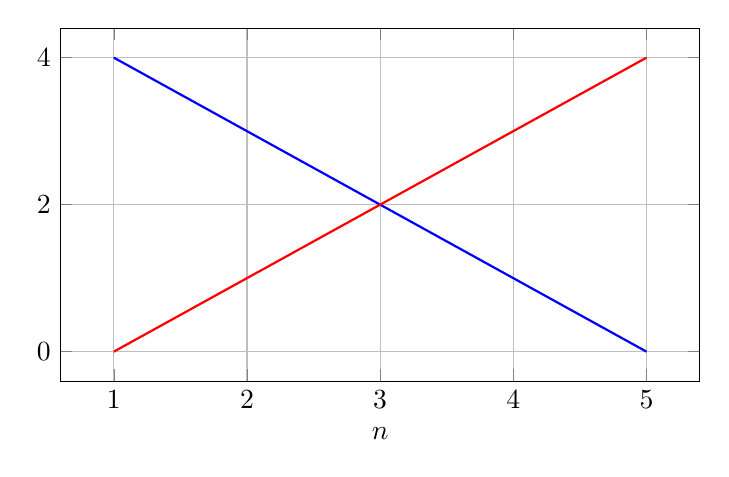
\begin{tikzpicture}
		\begin{axis}[
				xlabel={$n$},
				legend pos=outer north east,
				grid=major,
				width=0.8\textwidth,
				height=0.5\textwidth
			]
			\addplot[domain=1:5, samples=100, thick, blue] {5-x};
			\addplot[domain=1:5, samples=100, thick, red] {x-1};
		\end{axis}
	\end{tikzpicture}
	\caption{Plot of distance to road boundaries}
	\label{fig:road_boundaries}
\end{figure}

In this plot \ref{fig:road_boundaries}, the blue line represents \(\overline{n}(s) - n\), the red line represents \(n - \underline{n}(s)\).

We can also plot the objective function for the new formulation.

\begin{figure}[H]
	\centering
	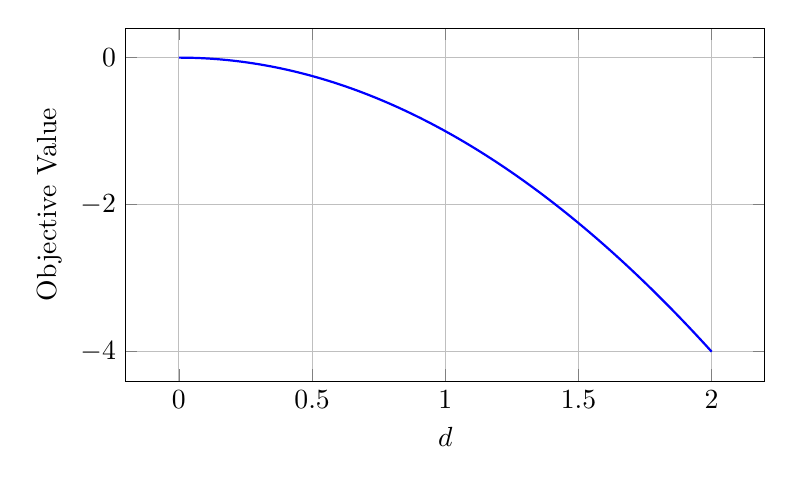
\begin{tikzpicture}
		\begin{axis}[
				xlabel={$d$},
				ylabel={Objective Value},
				legend pos=outer north east,
				grid=major,
				width=0.8\textwidth,
				height=0.5\textwidth
			]
			\addplot[domain=0:2, samples=100, thick, blue] {-x^2};
		\end{axis}
	\end{tikzpicture}
	\caption{Plot of the objective function}
	\label{fig:objective_functions}
\end{figure}

While \(-\min(5 - x, x - 1)\) is a convex function, it is piece wise linear, which can lead to difficulties in optimization.
The benefit of using an auxiliary variable in this context is that it allows us to transform a piece wise linear and potentially non-differentiable
objective function into a smooth and differentiable convex function.
This transformation simplifies the optimization process, making it more efficient and reliable.
Specifically, by introducing the auxiliary variable \( d \) and reformulating the objective as \(\min g(x, u) - d^2\), we obtain a function that is
easier to handle with gradient-based optimization algorithms, which rely on smoothness and differentiability to find optimal solutions effectively.

\subsection{Penalty Methods}

Penalty methods are another approach to handle constraints in optimization problems.
These methods incorporate constraints into the objective function by adding a penalty term that increases the objective value when constraints are
violated.
This approach transforms a constrained optimization problem into an unconstrained one, which can be easier to solve.

Consider an optimization problem with a constraint \( g(x) \leq 0 \).
In a penalty method, we modify the objective function to include a penalty term \( P(g(x)) \) that penalizes constraint violations.
A common choice for the penalty term is a quadratic function, such as \( P(g(x)) = \mu \max(0, g(x))^2 \), where \( \mu \) is a positive penalty
parameter.

The modified optimization problem can be written as:
\begin{align*}
	\min_{x} \quad & f(x) + \mu \max(0, g(x))^2
\end{align*}

By adjusting the value of \( \mu \), we can control the severity of the penalty for constraint violations.
A larger \( \mu \) places more emphasis on satisfying the constraint, while a smaller \( \mu \) allows for greater flexibility in violating the
constraint.

Penalty methods are particularly useful when dealing with complex constraints that are difficult to handle directly.
By incorporating these constraints into the objective function, we can leverage efficient unconstrained optimization algorithms to find solutions.

\subsection{Lagrangian Relaxation}

Lagrangian relaxation is a technique used to simplify complex optimization problems by relaxing some of the constraints and incorporating them into
the objective function using Lagrange multipliers.
This approach transforms the original problem into a simpler one that can be solved more easily.

Consider an optimization problem with a constraint \( g(x) \leq 0 \).
In Lagrangian relaxation, we introduce a Lagrange multiplier \( \lambda \geq 0 \) and form the Lagrangian function:
\[
	L(x, \lambda) = f(x) + \lambda g(x)
\]

The relaxed optimization problem can be written as:
\begin{align*}
	\min_{x} \quad          & L(x, \lambda)  \\
	\text{subject to} \quad & \lambda \geq 0
\end{align*}

By solving the relaxed problem for different values of \( \lambda \), we can obtain a lower bound on the optimal value of the original problem.
The quality of the bound depends on the choice of \( \lambda \), and finding the best value of \( \lambda \) is an optimization problem in itself.

Lagrangian relaxation is particularly useful in combinatorial optimization problems, where it can provide strong bounds and guide the search for
optimal solutions.
It is also a key component of more advanced techniques, such as the Lagrangian duality and the subgradient method.

\subsection{Conclusion}

In this chapter, we have explored various modeling techniques that are essential for solving complex optimization problems.
We discussed the use of soft constraints, auxiliary variables, penalty methods, and Lagrangian relaxation, each of which offers unique advantages for
handling different types of constraints and objectives.
By understanding and applying these techniques, we can formulate and solve optimization problems more effectively, leading to better solutions and
improved performance in practical applications.
